\documentclass[tikz,border=10pt]{standalone}
\usepackage{tikz}
\usetikzlibrary{shapes,arrows.meta,positioning,fit,backgrounds,calc}

% Styles
\tikzset{
  service/.style={rectangle, rounded corners, draw=black, very thick, minimum width=3.5cm, minimum height=1cm, align=center, fill=green!15},
  db/.style={cylinder, shape border rotate=90, draw=black, very thick, minimum height=1.2cm, minimum width=0.9cm, aspect=0.5, align=center, fill=orange!20},
  broker/.style={rectangle, draw=black, thick, minimum width=3cm, minimum height=0.9cm, align=center, fill=blue!15},
  arrow/.style={-{Latex[length=2.5mm,width=1.8mm]}, thick},
  component/.style={rectangle, draw=black!60, very thin, rounded corners, inner sep=6pt, fill=gray!10},
  cache/.style={rectangle, rounded corners, draw=red!60, thick, minimum width=2.5cm, minimum height=0.8cm, align=center, fill=red!10}
}

\begin{document}
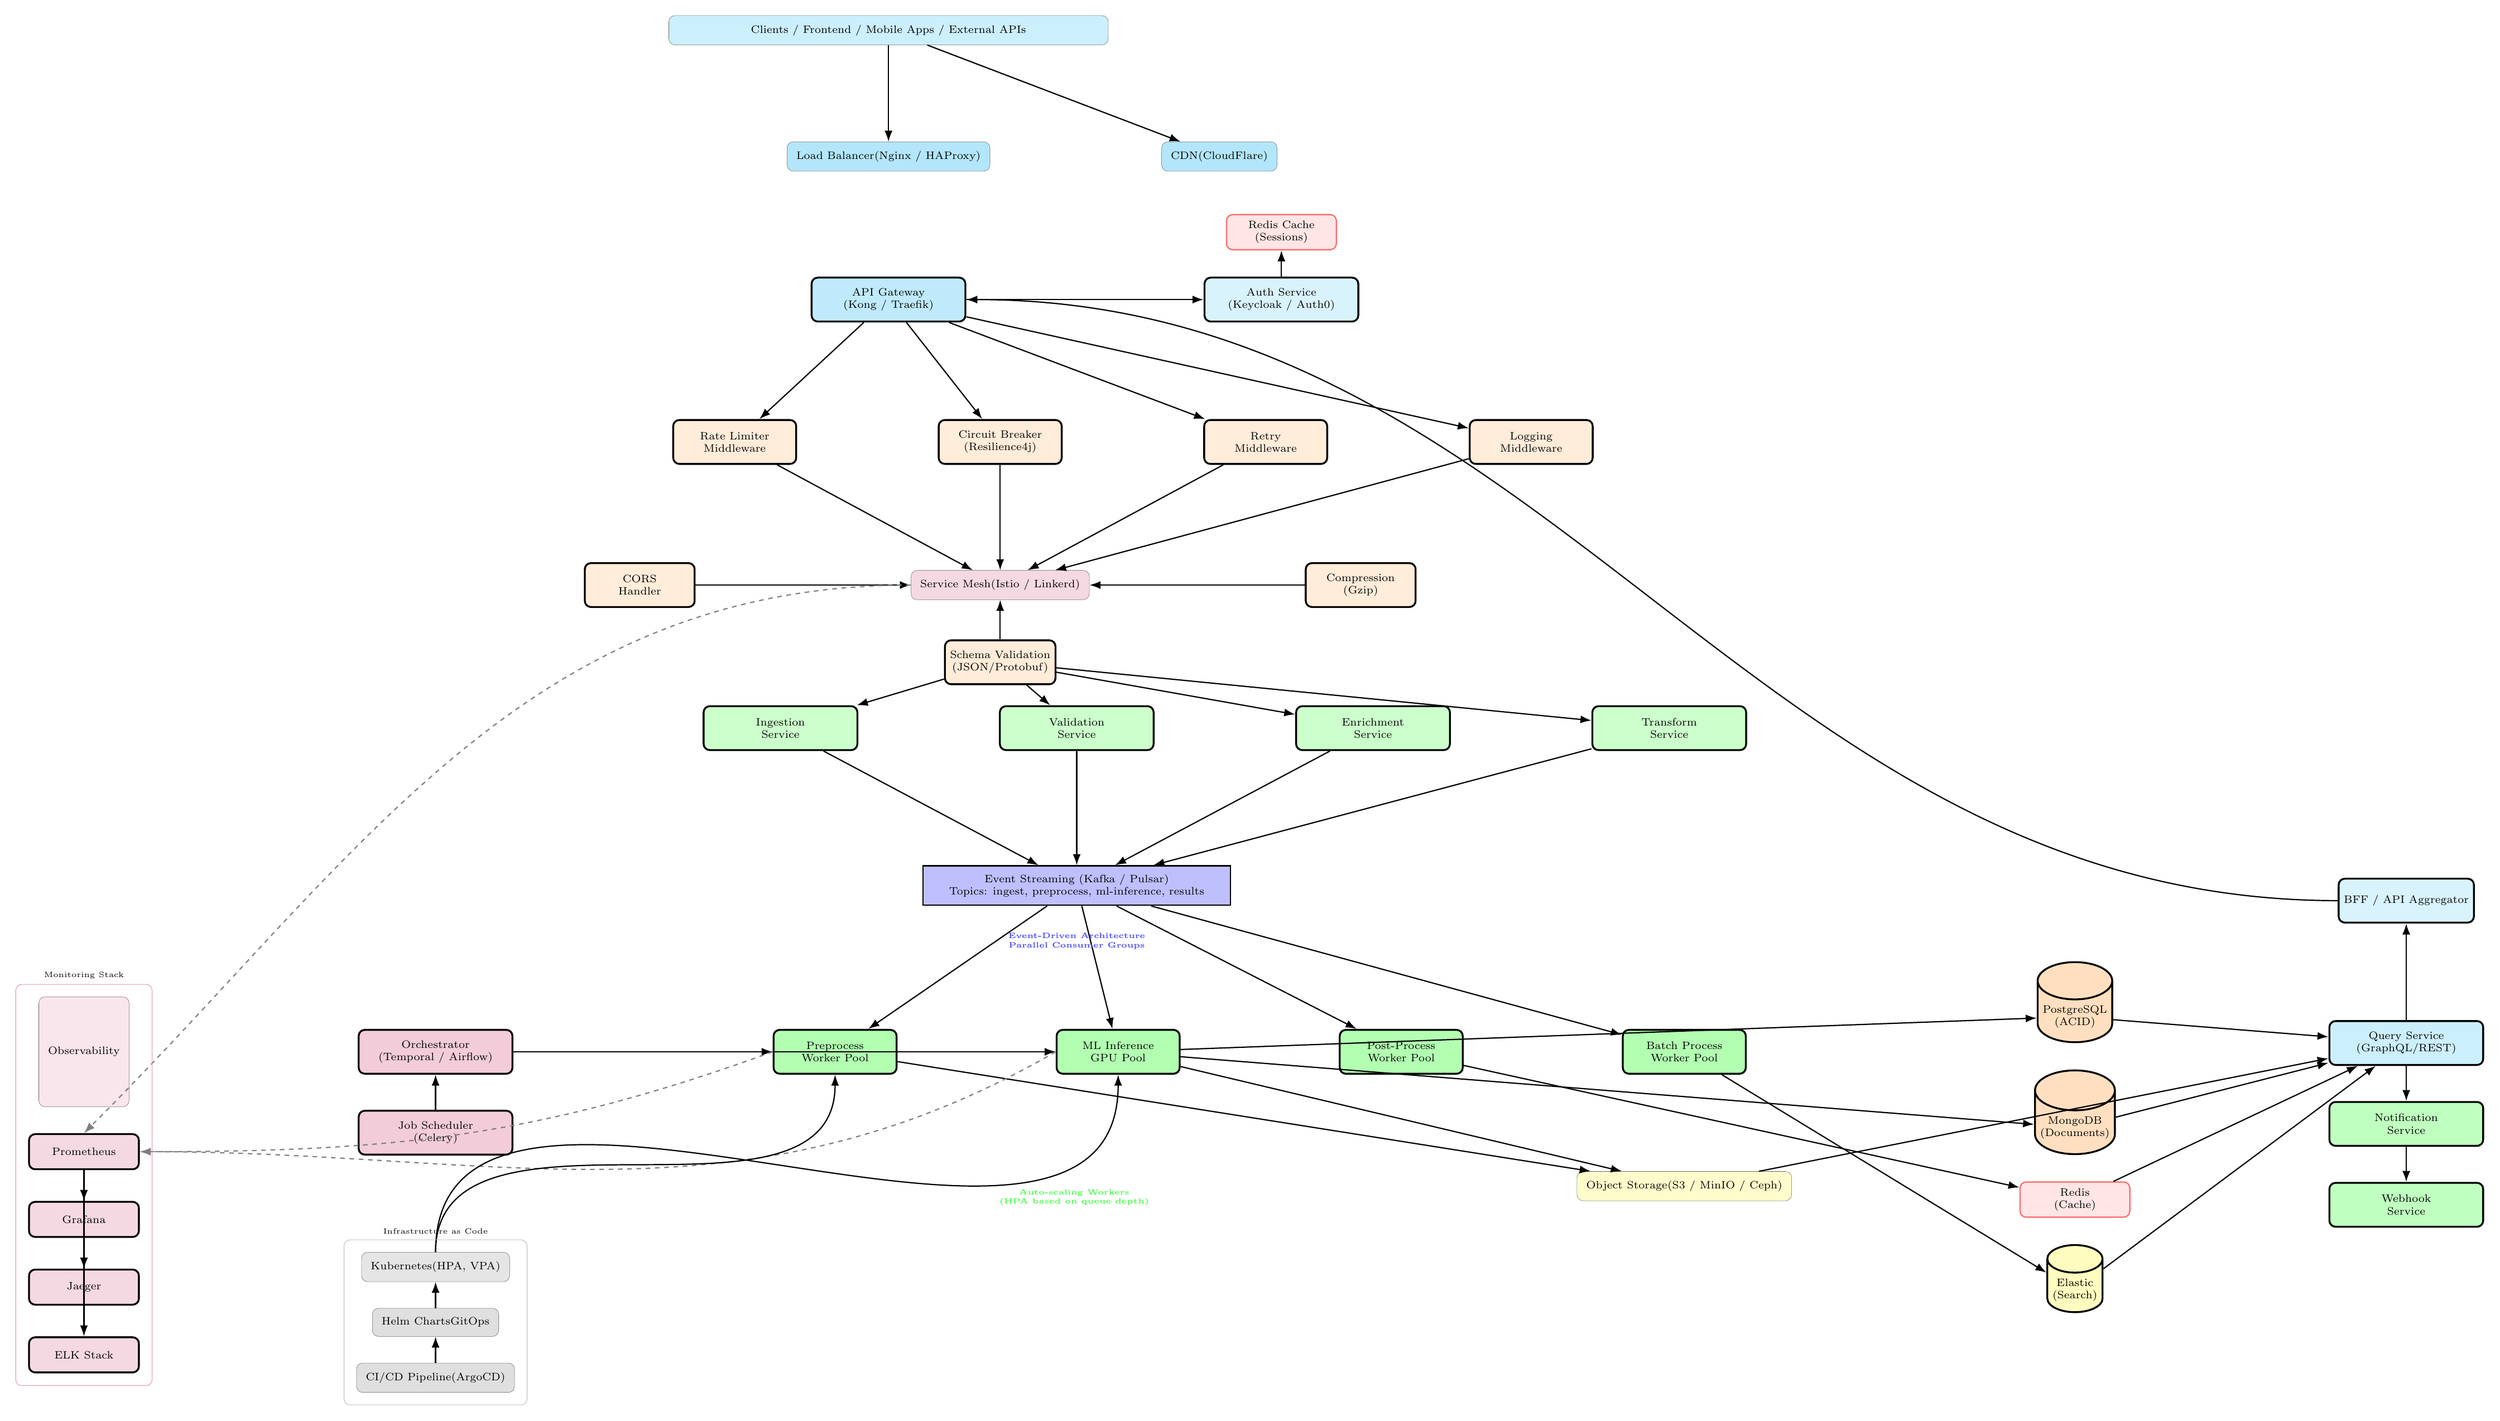
\begin{tikzpicture}[node distance=14mm and 24mm, every node/.style={font=\scriptsize}]

% Layer 1: External
\node (user) [component, fill=cyan!20, minimum width=10cm] {Clients / Frontend / Mobile Apps / External APIs};

% Layer 2: Edge Layer
\node (lb) [component, fill=cyan!30, below=of user, yshift=-8mm] {Load Balancer \\ (Nginx / HAProxy)};
\node (cdn) [component, right=of lb, xshift=15mm, fill=cyan!30] {CDN \\ (CloudFlare)};

% Layer 3: API Gateway + Auth + Middlewares
\node (gateway) [service, fill=cyan!25, below=of lb, yshift=-10mm] {API Gateway \\ (Kong / Traefik)};
\node (auth) [service, fill=cyan!15, right=of gateway, xshift=30mm] {Auth Service \\ (Keycloak / Auth0)};
\node (redis1) [cache, above=of auth, yshift=-8mm] {Redis Cache \\ (Sessions)};

% Middleware Layer
\node (ratelimit) [service, fill=orange!15, below=of gateway, yshift=-8mm, xshift=-35mm, minimum width=2.8cm] {Rate Limiter \\ Middleware};
\node (circuit) [service, fill=orange!15, right=of ratelimit, xshift=8mm, minimum width=2.8cm] {Circuit Breaker \\ (Resilience4j)};
\node (retry) [service, fill=orange!15, right=of circuit, xshift=8mm, minimum width=2.8cm] {Retry \\ Middleware};
\node (logging) [service, fill=orange!15, right=of retry, xshift=8mm, minimum width=2.8cm] {Logging \\ Middleware};

% Layer 4: Service Mesh + More Middlewares
\node (mesh) [component, fill=purple!15, below=of circuit, yshift=-10mm, minimum width=4cm] {Service Mesh \\ (Istio / Linkerd)};
\node (cors) [service, fill=orange!15, left=of mesh, xshift=-25mm, minimum width=2.5cm] {CORS \\ Handler};
\node (compress) [service, fill=orange!15, right=of mesh, xshift=25mm, minimum width=2.5cm] {Compression \\ (Gzip)};
\node (validation) [service, fill=orange!15, below=of mesh, yshift=5mm, minimum width=2.5cm] {Schema Validation \\ (JSON/Protobuf)};

% Layer 5: Core Services (Parallel Processing)
\node (ingest) [service, fill=green!20, below=of mesh, yshift=-10mm, xshift=-50mm] {Ingestion \\ Service};
\node (valid) [service, fill=green!20, right=of ingest, xshift=8mm] {Validation \\ Service};
\node (enrich) [service, fill=green!20, right=of valid, xshift=8mm] {Enrichment \\ Service};
\node (transform) [service, fill=green!20, right=of enrich, xshift=8mm] {Transform \\ Service};

% Layer 6: Message Broker (Event-Driven)
\node (kafka) [broker, below=of valid, yshift=-12mm, fill=blue!25, minimum width=7cm] {Event Streaming (Kafka / Pulsar) \\ Topics: ingest, preprocess, ml-inference, results};

% Layer 7: Processing Workers (Horizontal Scaling)
\node (preproc1) [service, below=of kafka, xshift=-55mm, yshift=-14mm, fill=green!30, minimum width=2.8cm] {Preprocess \\ Worker Pool};
\node (ml1) [service, right=of preproc1, xshift=12mm, fill=green!30, minimum width=2.8cm] {ML Inference \\ GPU Pool};
\node (postproc1) [service, right=of ml1, xshift=12mm, fill=green!30, minimum width=2.8cm] {Post-Process \\ Worker Pool};
\node (batch1) [service, right=of postproc1, xshift=12mm, fill=green!30, minimum width=2.8cm] {Batch Process \\ Worker Pool};

% Orchestration
\node (orchestrator) [service, left=of preproc1, xshift=-35mm, fill=purple!20] {Orchestrator \\ (Temporal / Airflow)};
\node (scheduler) [service, below=of orchestrator, yshift=6mm, fill=purple!20] {Job Scheduler \\ (Celery)};

% Layer 8: Data Layer
\node (postgres) [db, right=of batch1, xshift=42mm, yshift=8mm, fill=orange!25] {PostgreSQL \\ (ACID)};
\node (mongo) [db, below=of postgres, yshift=8mm, fill=orange!25] {MongoDB \\ (Documents)};
\node (redis2) [cache, below=of mongo, yshift=8mm] {Redis \\ (Cache)};
\node (elastic) [db, below=of redis2, yshift=8mm, fill=yellow!25] {Elastic \\ (Search)};

% Object Storage
\node (s3) [component, below=of batch1, yshift=-8mm, fill=yellow!20, minimum width=3cm] {Object Storage \\ (S3 / MinIO / Ceph)};

% Layer 9: Output Services
\node (query) [service, right=of postgres, xshift=25mm, yshift=-6mm, fill=cyan!20] {Query Service \\ (GraphQL/REST)};
\node (notify) [service, below=of query, yshift=6mm, fill=green!25] {Notification \\ Service};
\node (webhook) [service, below=of notify, yshift=6mm, fill=green!25] {Webhook \\ Service};

% BFF Layer
\node (bff) [service, above=of query, yshift=8mm, fill=cyan!15, minimum width=3cm] {BFF / API Aggregator};

% Layer 10: Observability Stack
\node (observ) [component, left=of orchestrator, xshift=-28mm, fill=purple!10, minimum height=2.5cm] {Observability};
\node (prom) [service, below=of observ, yshift=8mm, fill=purple!15, minimum width=2.5cm, minimum height=0.8cm] {Prometheus};
\node (graf) [service, below=of prom, yshift=7mm, fill=purple!15, minimum width=2.5cm, minimum height=0.8cm] {Grafana};
\node (jaeger) [service, below=of graf, yshift=7mm, fill=purple!15, minimum width=2.5cm, minimum height=0.8cm] {Jaeger};
\node (elk) [service, below=of jaeger, yshift=7mm, fill=purple!15, minimum width=2.5cm, minimum height=0.8cm] {ELK Stack};

% Infrastructure Layer
\node (k8s) [component, below=of scheduler, yshift=-8mm, fill=gray!20] {Kubernetes \\ (HPA, VPA)};
\node (helm) [component, below=of k8s, yshift=8mm, fill=gray!25] {Helm Charts \\ GitOps};
\node (ci) [component, below=of helm, yshift=8mm, fill=gray!25] {CI/CD Pipeline \\ (ArgoCD)};

% === ARROWS ===

% User to Edge
\draw[arrow] (user) -- (lb);
\draw[arrow] (user) -- (cdn);

% Gateway to Auth and Middlewares
\draw[arrow] (gateway) -- (auth);
\draw[arrow] (auth) -- (redis1);
\draw[arrow] (gateway) -- (ratelimit);
\draw[arrow] (gateway) -- (circuit);
\draw[arrow] (gateway) -- (retry);
\draw[arrow] (gateway) -- (logging);

% Middlewares to Service Mesh
\draw[arrow] (ratelimit) -- (mesh);
\draw[arrow] (circuit) -- (mesh);
\draw[arrow] (retry) -- (mesh);
\draw[arrow] (logging) -- (mesh);
\draw[arrow] (cors) -- (mesh);
\draw[arrow] (compress) -- (mesh);
\draw[arrow] (validation) -- (mesh);

% Mesh to Services
\draw[arrow] (validation) -- (ingest);
\draw[arrow] (validation) -- (valid);
\draw[arrow] (validation) -- (enrich);
\draw[arrow] (validation) -- (transform);

% Services to Kafka
\draw[arrow] (ingest) -- (kafka);
\draw[arrow] (valid) -- (kafka);
\draw[arrow] (enrich) -- (kafka);
\draw[arrow] (transform) -- (kafka);

% Kafka to Workers
\draw[arrow] (kafka) -- (preproc1);
\draw[arrow] (kafka) -- (ml1);
\draw[arrow] (kafka) -- (postproc1);
\draw[arrow] (kafka) -- (batch1);

% Orchestrator
\draw[arrow] (orchestrator) -- (preproc1);
\draw[arrow] (orchestrator) -- (ml1);
\draw[arrow] (scheduler) -- (orchestrator);

% Workers to Storage
\draw[arrow] (preproc1) -- (s3);
\draw[arrow] (ml1) -- (postgres);
\draw[arrow] (ml1) -- (mongo);
\draw[arrow] (postproc1) -- (redis2);
\draw[arrow] (batch1) -- (elastic);
\draw[arrow] (ml1) -- (s3);

% Storage to Query Services
\draw[arrow] (postgres) -- (query);
\draw[arrow] (mongo) -- (query);
\draw[arrow] (redis2) -- (query);
\draw[arrow] (elastic) -- (query);
\draw[arrow] (s3) -- (query);

% Query to Output
\draw[arrow] (query) -- (bff);
\draw[arrow] (query) -- (notify);
\draw[arrow] (notify) -- (webhook);

% BFF back to Gateway
\draw[arrow] (bff) to[out=180,in=0] (gateway);

% Observability connections
\draw[arrow, dashed, gray] (mesh.west) to[out=180,in=45] (prom.north);
\draw[arrow, dashed, gray] (preproc1.west) to[out=200,in=0] (prom.east);
\draw[arrow, dashed, gray] (ml1.west) to[out=210,in=0] (prom.east);
\draw[arrow] (prom) -- (graf);
\draw[arrow] (prom) -- (jaeger);
\draw[arrow] (graf) -- (elk);

% Infrastructure
\draw[arrow] (k8s.north) to[out=90,in=270] (preproc1.south);
\draw[arrow] (k8s.north) to[out=90,in=270] (ml1.south);
\draw[arrow] (helm) -- (k8s);
\draw[arrow] (ci) -- (helm);

% Annotations
\node[align=center, font=\tiny\bfseries, text=blue!70] at ($(kafka.south)+(0,-0.8)$) {Event-Driven Architecture \\ Parallel Consumer Groups};

\node[align=center, font=\tiny\bfseries, text=green!70] at ($(ml1.south)+(-1,-2.8)$) {Auto-scaling Workers \\ (HPA based on queue depth)};

% Grouping boxes
\node[draw=purple!40, rounded corners, fit=(prom) (graf) (jaeger) (elk) (observ), inner sep=8pt, label={[font=\tiny]above:Monitoring Stack}] {};

\node[draw=gray!50, rounded corners, fit=(k8s) (helm) (ci), inner sep=8pt, label={[font=\tiny]above:Infrastructure as Code}] {};

\end{tikzpicture}
\end{document}
